\documentclass[UTF8]{ctexart}
\ctexset{
  section={
    format=\raggedright\zihao{3},
    name={T,}
  },
  subsection={
    format={\zihao{4}},
    number={\arabic{subsection}}
  }
}
\usepackage[a4paper,left=3cm,right=3cm,top=2cm]{geometry}
\usepackage{amsmath}
\usepackage{enumitem}
\usepackage{float}
\usepackage{threeparttable}
\usepackage{caption}
\usepackage{multirow}
\usepackage{graphicx}
\usepackage{listings}
\usepackage{color}

\definecolor{dkgreen}{rgb}{0,0.6,0}
\definecolor{gray}{rgb}{0.5,0.5,0.5}
\definecolor{mauve}{rgb}{0.58,0,0.82}
\lstset{frame=tb,
  language=C,
  aboveskip=3mm,
  belowskip=3mm,
  showstringspaces=false,
  columns=flexible,
  basicstyle={\small\ttfamily},
  numbers=left,%设置行号位置none不显示行号
  %numberstyle=\tiny\courier, %设置行号大小
  numberstyle=\color{gray},
  keywordstyle=\color{blue},
  commentstyle=\color{dkgreen},
  stringstyle=\color{mauve},
  breaklines=true,
  breakatwhitespace=true,
  escapeinside=`,%逃逸字符(1左面的键),用于显示中文例如在代码中`中文...`
  tabsize=4,
  extendedchars=false %解决代码跨页时,章节标题,页眉等汉字不显示的问题
}

\setlength\lineskiplimit{5.25bp}
\setlength\lineskip{5.25bp}

\title{ICS Homework 2}
\author{崔士强 PB22151743}
\date{\today}

\bibliographystyle{plain}

\begin{document}

\maketitle
\section{}  % T1
左上:C

左下:C    

右上:A    

右下:A 

\begin{table}[H]\centering
  \setlength{\tabcolsep}{8mm}
  \begin{tabular}{ccc|c}
    \hline\hline
    A & B & C & Y \\
    \hline
    0 & 0 & 0 & 1 \\
    0 & 0 & 1 & 1 \\
    0 & 1 & 0 & 1 \\
    0 & 1 & 1 & 0 \\
    1 & 0 & 0 & 1 \\
    1 & 0 & 1 & 0 \\
    1 & 1 & 0 & 1 \\
    1 & 1 & 1 & 0 \\
    \hline\hline
  \end{tabular}
  \caption{真值表}
\end{table}
\section{}  % T2
如下图所示,NAND可以组成非门,从而组成与门,进一步组成或门。由于与门,非门,或门逻辑完备,因此NAND门也是逻辑完备的。
\clearpage
\begin{figure}[h]
  \centering
  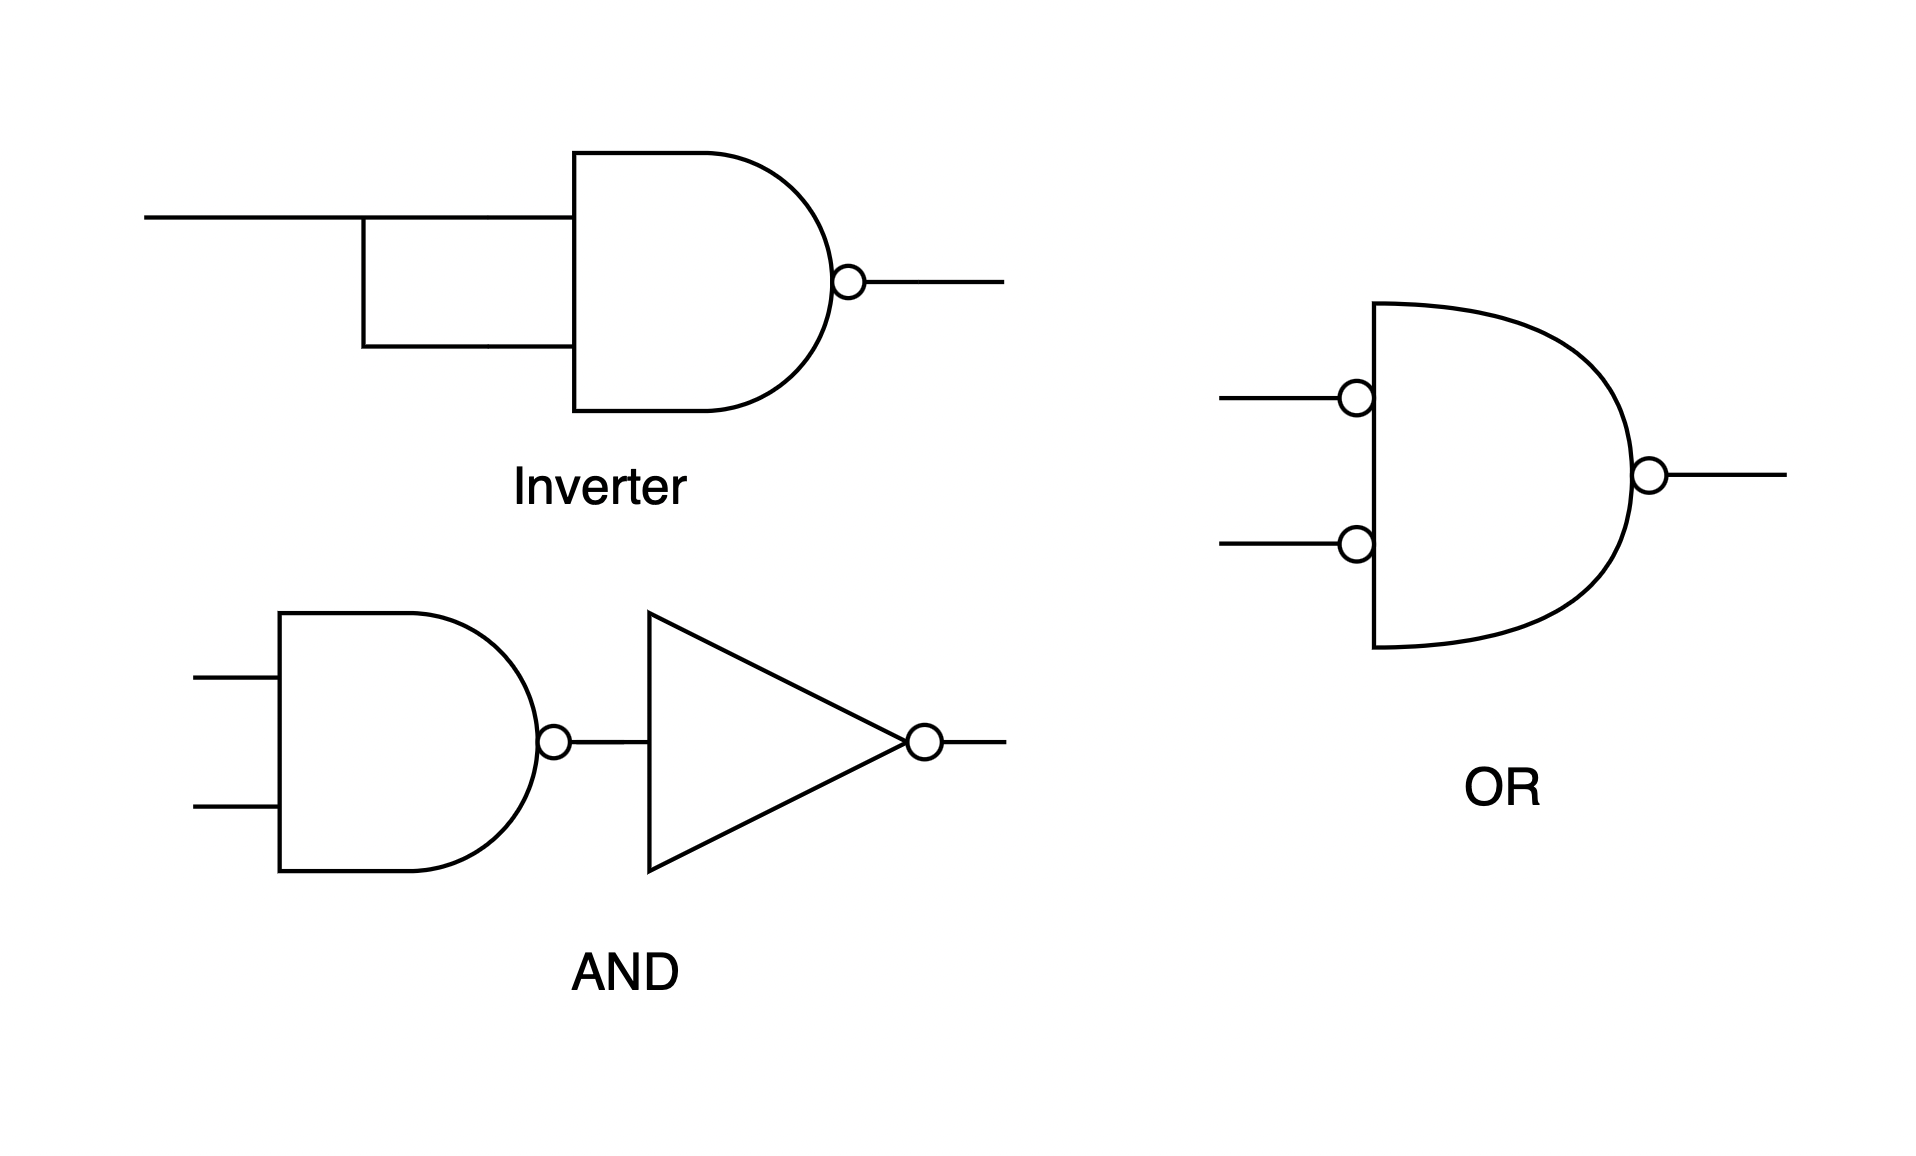
\includegraphics[scale=0.3]{p1.png}
  \caption{T2}
\end{figure}
\section{}  % T3
\begin{figure}[h]
  \centering
  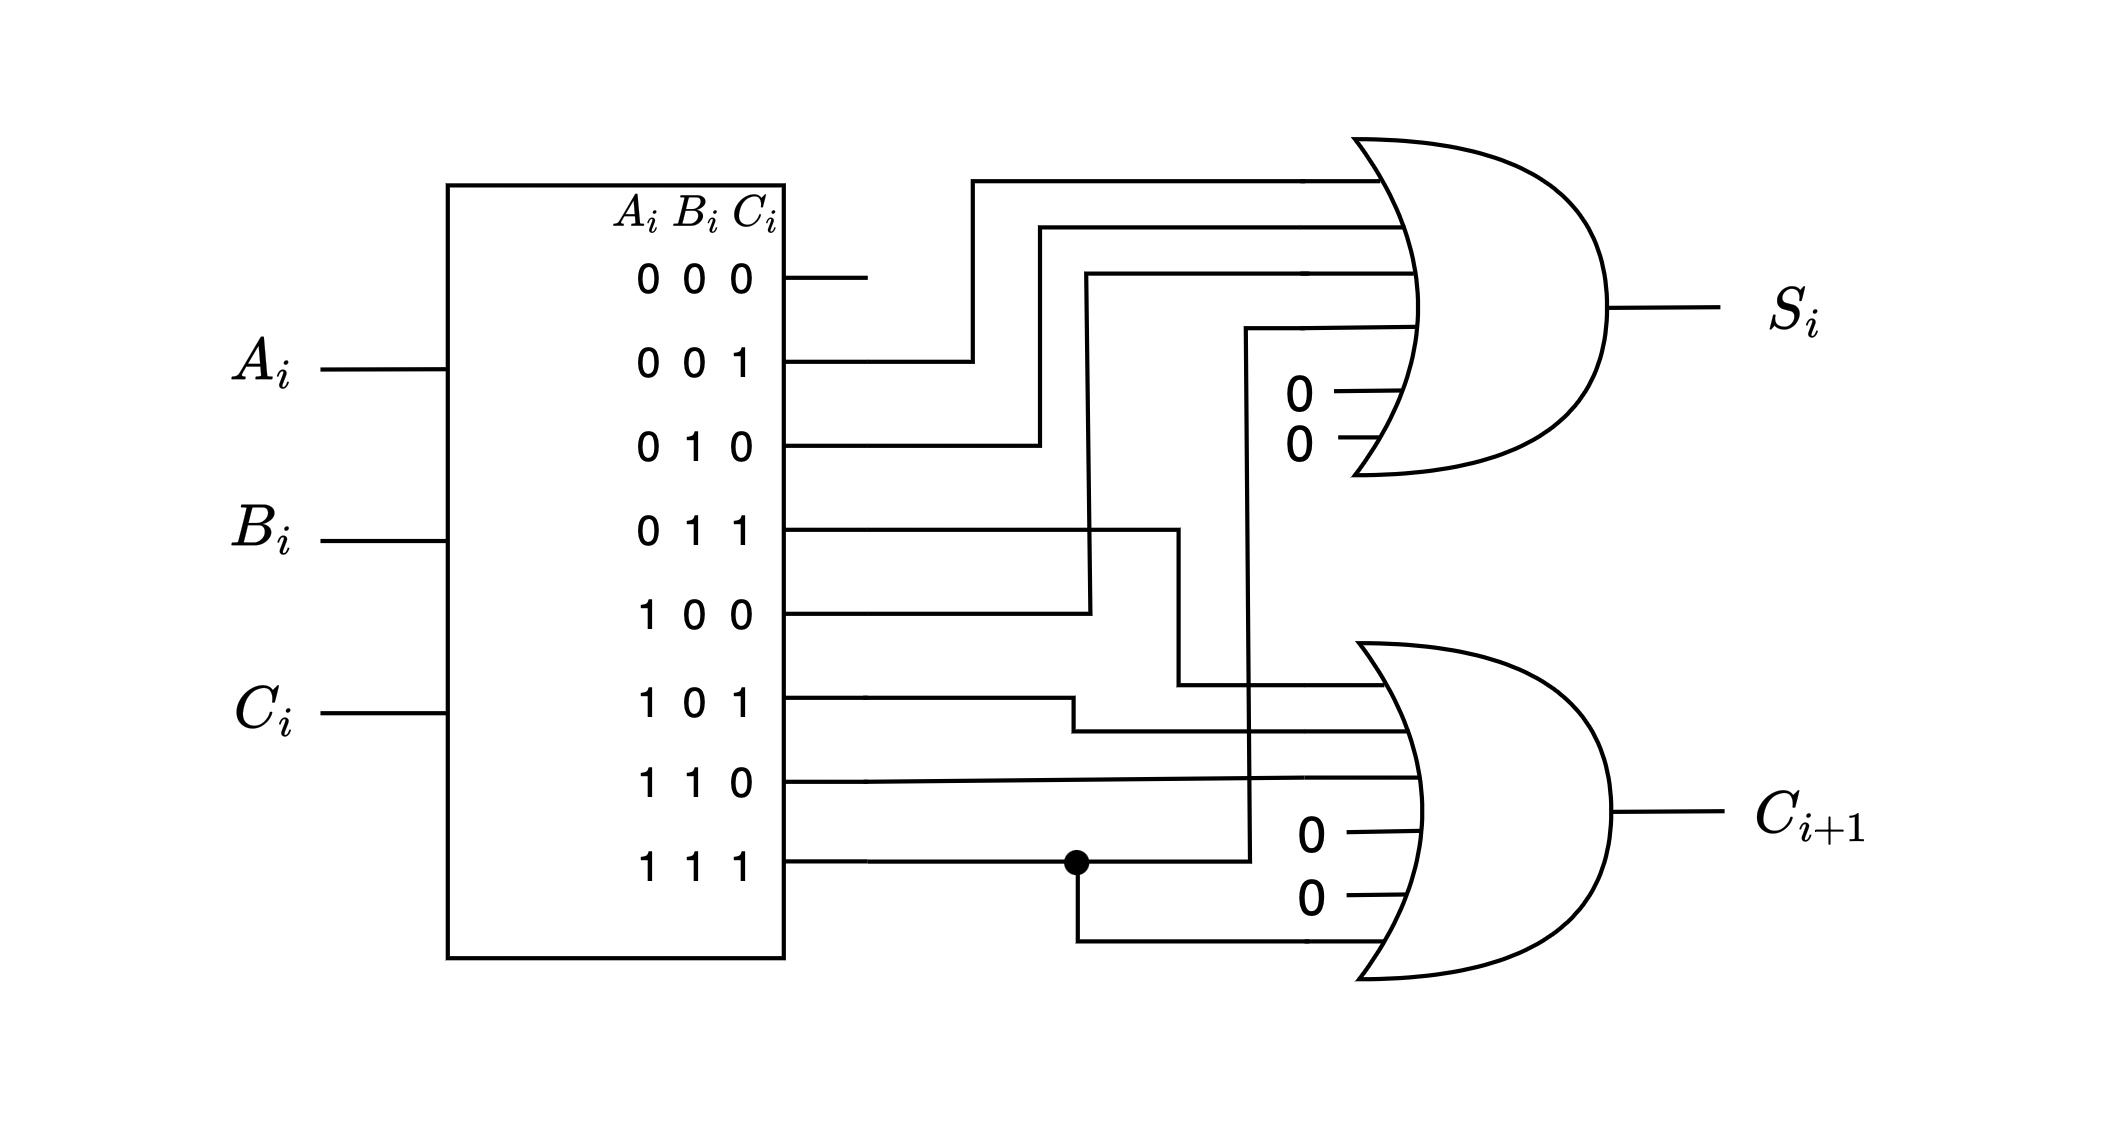
\includegraphics[scale=0.3]{p2.png}
  \caption{T3}
\end{figure}
\section{}  % T4
\begin{enumerate}
  \item 3
  \item 3
  \item 9
  \item 4
  \item 如下表所示
\begin{table}[H]\centering
  \begin{tabular}{cccc|cccc}
    \hline\hline
    $A[1]$ & $A[0]$ & $B[1]$ & $B[0]$ & $Y[3]$ & $Y[2]$ & $Y[1]$ & $Y[0]$ \\
    \hline
    0 & 0 & 0 & 0 & 0 & 0 & 0 & 0 \\
    0 & 0 & 0 & 1 & 0 & 0 & 0 & 0 \\
    0 & 0 & 1 & 0 & 0 & 0 & 0 & 0 \\
    0 & 0 & 1 & 1 & 0 & 0 & 0 & 0 \\
    0 & 1 & 0 & 0 & 0 & 0 & 0 & 0 \\
    0 & 1 & 0 & 1 & 0 & 0 & 0 & 1 \\
    0 & 1 & 1 & 0 & 0 & 0 & 1 & 0 \\
    0 & 1 & 1 & 1 & 0 & 0 & 1 & 1 \\
    1 & 0 & 0 & 0 & 0 & 0 & 0 & 0 \\
    1 & 0 & 0 & 1 & 0 & 0 & 1 & 0 \\
    1 & 0 & 1 & 0 & 0 & 1 & 0 & 0 \\
    1 & 0 & 1 & 1 & 0 & 1 & 1 & 0 \\
    1 & 1 & 0 & 0 & 0 & 0 & 0 & 0 \\
    1 & 1 & 0 & 1 & 0 & 0 & 1 & 1 \\
    1 & 1 & 1 & 0 & 0 & 1 & 1 & 0 \\
    1 & 1 & 1 & 1 & 1 & 0 & 0 & 1 \\
    \hline
  \end{tabular}
\end{table}
  \item
$$Y[2]=A[1]\overline{A[0]}B[1]\overline{B[0]} + A[1]\overline{A[0]}B[1]B[0] + A[1]A[0]B[1]\overline{B[0]}$$
\end{enumerate}
\section{}  % T5
\begin{figure}[h]
  \centering
  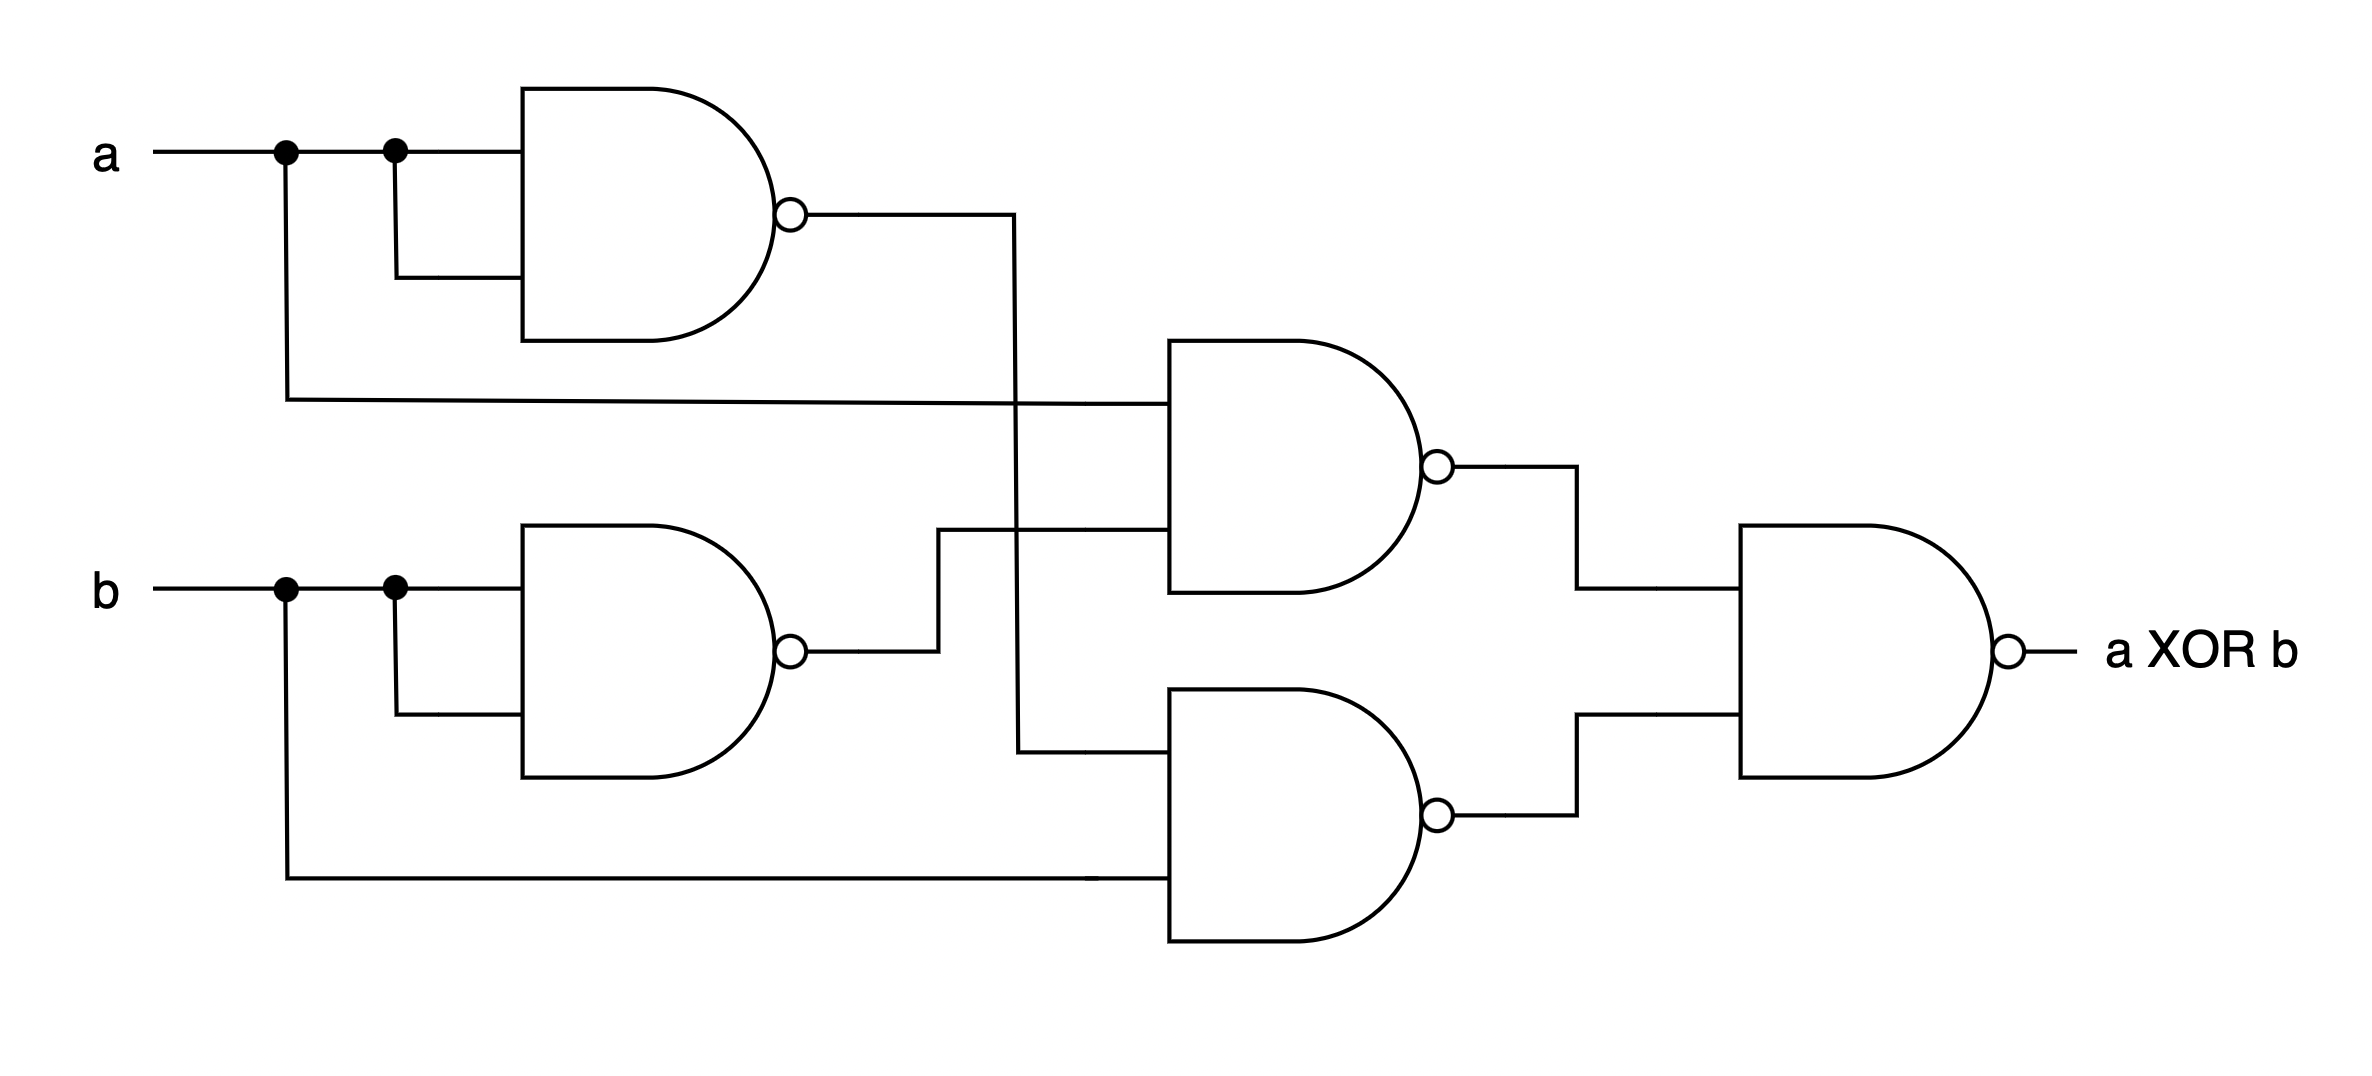
\includegraphics[scale=0.3]{p4.png}
  \caption{T5}
\end{figure}
\section{}  % T6
\begin{table}[H]\centering
  \setlength{\tabcolsep}{8mm}
  \begin{tabular}{cccc|c}
    \hline\hline
    A & B & C & D & Y\\
    \hline
    0 & 0 & 0 & 0 & 0 \\
    0 & 0 & 0 & 1 & 0 \\
    0 & 0 & 1 & 0 & 0 \\
    0 & 0 & 1 & 1 & 0 \\
    0 & 1 & 0 & 0 & 0 \\
    0 & 1 & 0 & 1 & 0 \\
    0 & 1 & 1 & 0 & 1 \\
    0 & 1 & 1 & 1 & 0 \\
    1 & 0 & 0 & 0 & 1 \\
    1 & 0 & 0 & 1 & 0 \\
    1 & 0 & 1 & 0 & 0 \\
    1 & 0 & 1 & 1 & 0 \\
    1 & 1 & 0 & 0 & 0 \\
    1 & 1 & 0 & 1 & 0 \\
    1 & 1 & 1 & 0 & 0 \\
    1 & 1 & 1 & 1 & 0 \\
    \hline\hline
  \end{tabular}
  \caption{真值表}
\end{table}
\begin{figure}[h]
  \centering
  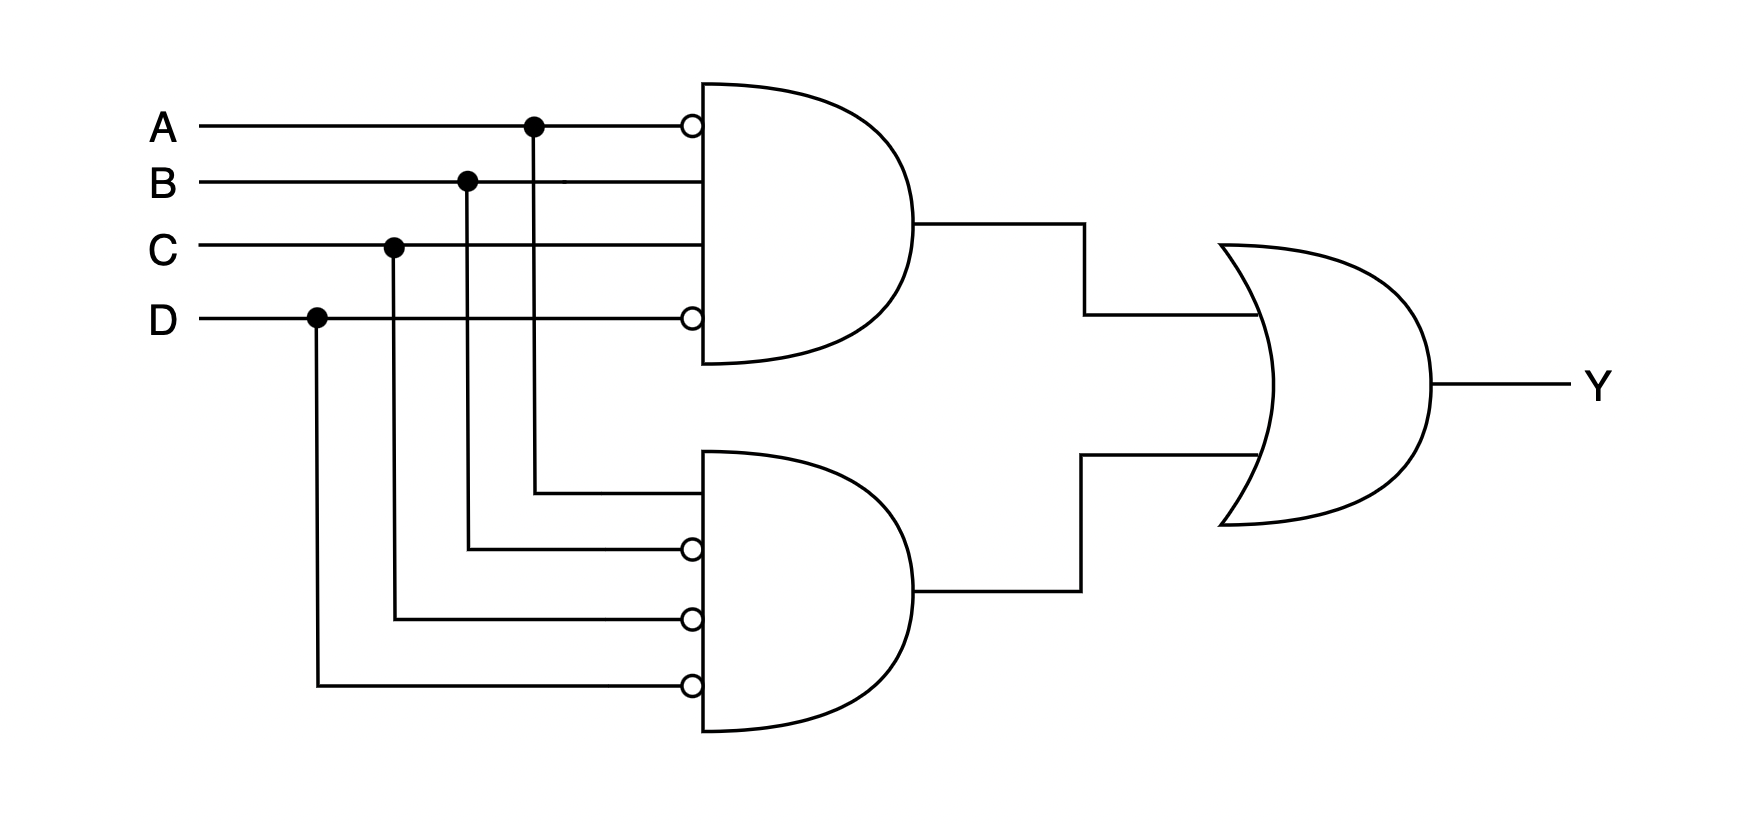
\includegraphics[scale=0.3]{p3.png}
  \caption{T6}
\end{figure}
\clearpage
\section{}  % T7
\begin{enumerate}
  \item 如下图所示
  \begin{figure}[h]
    \centering
    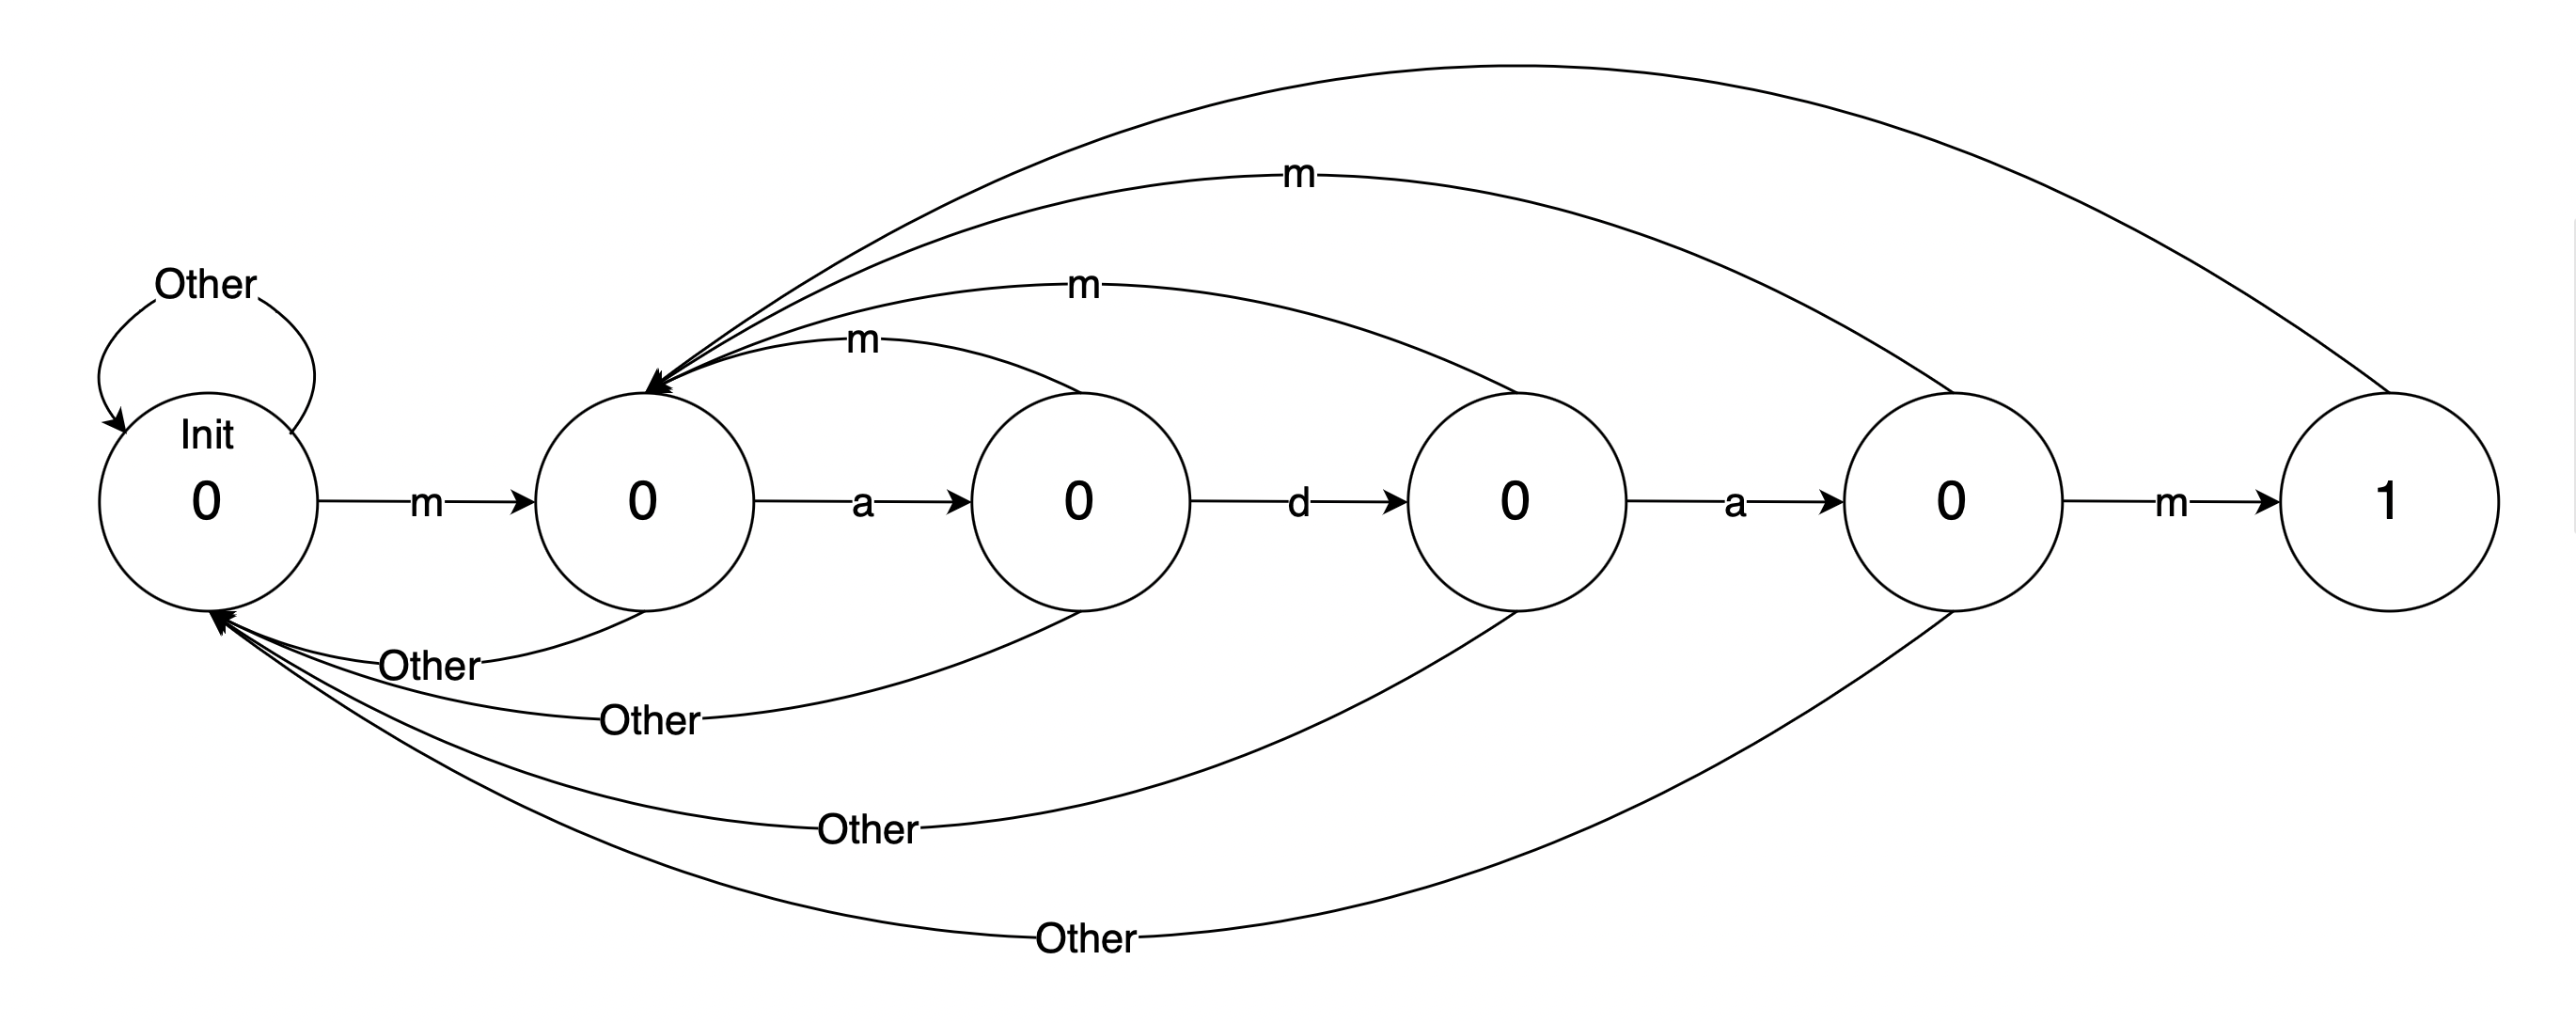
\includegraphics[scale=0.3]{p5.png}
    \caption{T7}
  \end{figure}
  \item 6
\end{enumerate}
\section{}  % T8
\begin{enumerate}
  \item $2^a$
  \item $2^ab$
\end{enumerate}
\section{}  % T9
\begin{enumerate}
  \item $A[1:0]=0, WE=1$
  \item 在每一行增加Gated D-latch,并将D[2:0]扩展到D[k-1:0]
  \item 
\end{enumerate}
\section{}  % T10
\begin{enumerate}
  \item 
  \item $$2\times 7 + 2\times 2 + \left(2 + 6\right) + 8\times 7 = 78$$ 
\end{enumerate}
\bibliography{math}

\end{document}
\iffalse
\begin{figure}[h]
    \centering
    \includegraphics[scale=0.5]{name.png}
    \caption{name}
\end{figure}
\fi